\subsection{Satisfiability Modulo Theories Solvers}
In relation to the Satisfiability Solvers, the Satisfiablity Modulo Theories solvers, short SMT solvers, take a step back. Because it is often time consuming to formulate your domain specific problem as a boolean formula and transform it into CNF. In this section an overview over how STP \cite{Ganesh:2007:DPB:1770351.1770421}, which is used in KLEE and other tools, works is given.\\
In contrast to SAT solvers, STP is able to solve decision problems that contain bit-vectors and arrays. Which in practise allows us to reason about various data types such as integers, integers are principally bit vectors and also some datastructures like lists and arrays.\\
As an input STP allows the following operations, which can be grouped in the following way:\\
\begin{itemize}
\item \textbf{logical and boolean} Constant Values TRUE and FALSE, variables with a boolean value, any boolean operator\footnote{such as $\lor$,$\land$, $\Rightarrow$, etc}, bitwise boolean operators \\
\item \textbf{mathematic operations} Left and right shifts, addition, multiplication, unary minus, division, modulo, relational operators\\
\item \textbf{others} Array read, array write,  extraction of bit-vectors\footnote{$x[i:j]$ is the extraction of the bytes between $i$ and $j$ of $x$}, concatenation of bit-vectors\footnote{The concatenation of two bit-vectors $x_{[n]}$ and $y_{[m]}$ is expressed as $x \circ y$ and returns a new vector $z_{[m+n]}$ of length $m+n$}\\
\end{itemize}
STP was specifically developed with focus on software analysis projects, because there are often extremely large constraint problems involved. In relation to other SMT solvers STP focuses on reducing the size of a quantifier-freee first order logic problem, until it can be converted into conjunctive normal form and therefore be solved by a SAT solver, which allows it to benefit from the heavely engineered and therefore very fast SAT solvers. Other SMT solvers apply the theory specific decision procedures not until in the SAT solver, which often leads to problems with the SAT specific optimizations.The architecture of STP is visualized in the figure \ref{fig:spt_architecture}.
TODO add more content about the general working of STP, especially the array refinement
To reduce the size of a problem it applies optimations specific to bit-vector and array theory.
\begin{figure}
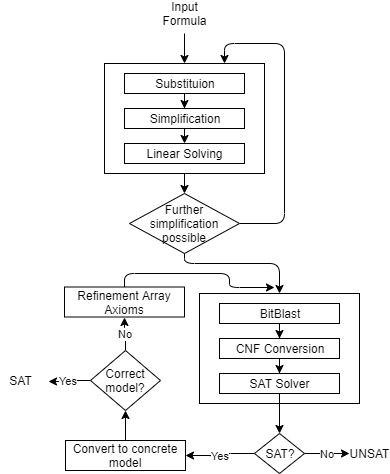
\includegraphics[width=\linewidth]{SPT_architecture}
\centering
\caption{SPT Architecture}
\label{fig:spt_architecture}
\end{figure}
In the original paper\cite{Ganesh:2007:DPB:1770351.1770421} there are two of these optimizations discussed. The first optimization is an "on-the-fly solver for mod-$2^n$ linear arithmetic", which is embedded in STP. 
When reasoning about fixed length bit-vector arithmetic this part of the program tries to reason about parts of the bit-vector equality system.
The idea is to use the property of a such a vector that you can always calculate in $\mod{2^b}$ where is b is the length of the bit-vector.
There exists a mathematical theorem in basic number theory which can be used to determine if a solution to an equation exists if it is$\mod{2^b}$:
$$\sum_{i=1}^{n} a_ix_i = c_i  \Mod{2^b}$$
$$gcd(a_1,...,a_n,2^b) | c_i$$
The equation is only solvable if the greatest common divisor, also known as gcd, is a divisor of every $c_i$.\
Lets assume the following equality system where all variables are bit-vectors with length 3, $b$ is therefore 3:
TODO replace system with own example
$$3x+4y+2z=0 \Mod{2^3}$$
$$2x+2y+2=0  \Mod{2^3}$$
$$2x+4y+2z=0 \Mod{2^3}$$
If we know that the $gcd$ of two numbers is $a$ and $m$ is 1, $a$ has per definition a multiplicative inverse in mod $m$. In this case we are interested in $m=2^b$. This property is necessary, because we need to isolate one of the variables and therefore multiply with the inverse\footnote{This is neccessary because division in modular arithmetic is not defined and replaced with the multiplication of the inverse}.
The algorithm chooses the first equation and tries to find an $a_i$ where $gcd(a_i,2^3) = 1$ is true. In our example it finds $a_1$ which has the value $3$, therefore we are able to isolate x in the first equation.
The first step is to multiple with the multiplicative inverse of 3 in$\mod{2^3}$ which is also 3.
$$3x+4y+2z = 0 \Mod{2^3} \xleftrightarrow{\text{isolate 3x}}$$
$$3x=-4y-2z  \Mod{2^3}   \xleftrightarrow{\text{normalize to mod8}}$$
$$3x=4y+6z  \Mod{2^3}  \xleftrightarrow{\text{multiple with 3}}$$
$$x=12y+18z \Mod{2^3}  \xleftrightarrow{\text{normalize to mod8}}$$
$$x=4y+2z \Mod{2^3} $$
After we isolated $x$ we can substitute each $x$ in the original equality system with $4y+2z$
$$2(\underbrace{4y+2z}_{x})+2y+2=0 \Mod{2^3} \Leftrightarrow 2y + 4z + 2 = 0\Mod{2^3} $$
$$2(\underbrace{4y+2z}_{x})+ 4y + 2z = 0 \Mod{2^3} \Leftrightarrow 4y + 6z = 0\Mod{2^3} $$
There are no longer any ${a_i}$ in these equalities, that have an $gcd(a_i,2^3)$ and therefore no further variable can be isolated.
The algorithm then searches the coefficent $a_i$ which is the smallest over the whole system and chooses the belonging equality.
After the smallest $a_i$ is choosen the whole system is devided by it and the bit with the highest order is dropped.
A whole new equality system is formed with linear vectors length $b-1$, in the example two.
The new variables are named $y[1:0]$ and $z[1:0]$ to signal that they represent the bits 1 to 0 of the regarding variable.
$$y[1 : 0] + 2z[1 : 0] + 1 = 0 \Mod{2^2}$$
$$2y[1 : 0] + 3z[1 : 0] = 0\Mod{2^2}$$
Now the first step of isolation a variable $x_i$ with a coefficient $gcd(a_i, 2^b)=1$ is repeated.
$$y[1 : 0] + 2z[1 : 0] + 1 = 0 \Mod{2^2} \xleftrightarrow{\text{isolate y[1:0]}}$$
$$y[1 : 0] = -2z[1 : 0] -1 \Mod{2^2} \xleftrightarrow{\text{normalize to mod4}}$$
$$y[1 : 0] = 2z[1 : 0] +3 \Mod{2^2} \xleftrightarrow{\text{normalize to mod4}}$$
After we isolated $y[1 : 0] $ we can substitute each $y[1 : 0] $ in the original equality system with $2z[1:0]+3$
$$2(\underbrace{2z[1:0]+3}_{y[1:0]}) + 3z[1 : 0] = 0\Mod{2^2} \xleftrightarrow{\text{normalize to mod4}}$$
$$3z[1:0] + 2 = 0 \Mod{2^2}$$
In the last iteration we can isolate $z[1:0]$ because the $gcd(3,2^2) = 1$. The inverse of 3 in $\mod{2^2}$ is 3.
$$3z[1:0] + 2 = 0 \Mod{2^2} \xleftrightarrow{\text{isolate 3z[1:0]}}$$
$$3z[1:0]=-2  \Mod{2^2}   \xleftrightarrow{\text{normalize to mod4}}$$
$$3z[1:0]=2  \Mod{2^2}   \xleftrightarrow{\text{multiple with 3}}$$
$$z[1:0]=6  \Mod{4}  \xleftrightarrow{\text{normalize to mod4}}$$
$$z[1:0]=2  \Mod{4}$$
Because we got a solution we can conclude that the original equation system is satisfiable.
The original system can be transformed into $$(x = 4y + 6z) \land (y[1 : 0] = 2z[1 : 0] + 3) \land (z[1 : 0] = 2)$$ and forwarded to the SAT solver.

TODO cleanup
How SMT solvers work in comparison to SAT solvers.
Especially how the STP \cite{Ganesh:2007:DPB:1770351.1770421} (used in KLEE and other tools) works.
Basically by transforming the input and solve the result of the transformation, if neccessary, with a SAT solver.
Description of Bit-Vector Arithmentic used in the on-the-fly solver\cite{10.1007/978-3-540-71209-1_28}
STP uses many different algorithms to optimize the formula. In the next section two of these optimizations are described, as an example.
on-the-fly solver for mod-2n linear arithmetic
abstraction refinement heuristics for array expressions 